\documentclass[10pt,a4paper]{article}

\usepackage[a4paper]{geometry}
\usepackage[hidelinks]{hyperref}
\usepackage{graphicx}
\usepackage{pdfpages}

\newcommand\blankpage{
    \null
    \thispagestyle{empty}
    % \addtocounter{page}{-1}%
    \newpage}

\begin{document}

\pagenumbering{roman}

\newgeometry{top=3cm}
\begin{titlepage}

\center

\begin{minipage}{0.5\textwidth}
\begin{flushleft}

\includegraphics[scale=0.25]{univ-luxembourg-logo.eps}
\end{flushleft}
\end{minipage}
~
% Logo of the hosting institution? Put it here.
\begin{minipage}{0.4\textwidth}
\begin{flushright}
% \includegraphics[scale=0.6]{other-logo.png}
\end{flushright}
\end{minipage}
\\[2cm]

{ \LARGE \textsc{Title of your Master Thesis}}\\[2cm]

      Author\\[2mm]
      {\large \textsc Your Name}\\[1cm]
      \vskip 1cm
      Supervised by\\[2mm]
      {\large \textsc Prof. High Perf, affiliation\\[1mm]
       \large \textsc Dr. Low Perf, affiliation
      % add/remove supervisors if needed
      }\\[1cm]
      Reviewed by\\[2mm]
      {\large \textsc Dr. Slurm, affiliation}\\[1cm]
      Examined by\\[2mm]
      {\large \textsc Dr. Slurm, affiliation}\\[1cm]

\vfill % Fill the rest of the page with whitespace
A Thesis submitted in fulfillment of requirements for the degree of\\[0.1cm]
\textbf{Master in High Performance Computing}\\[0.7cm]

Department of Computer Science\\
University of Luxembourg\\
2025

\end{titlepage}

\restoregeometry

\blankpage
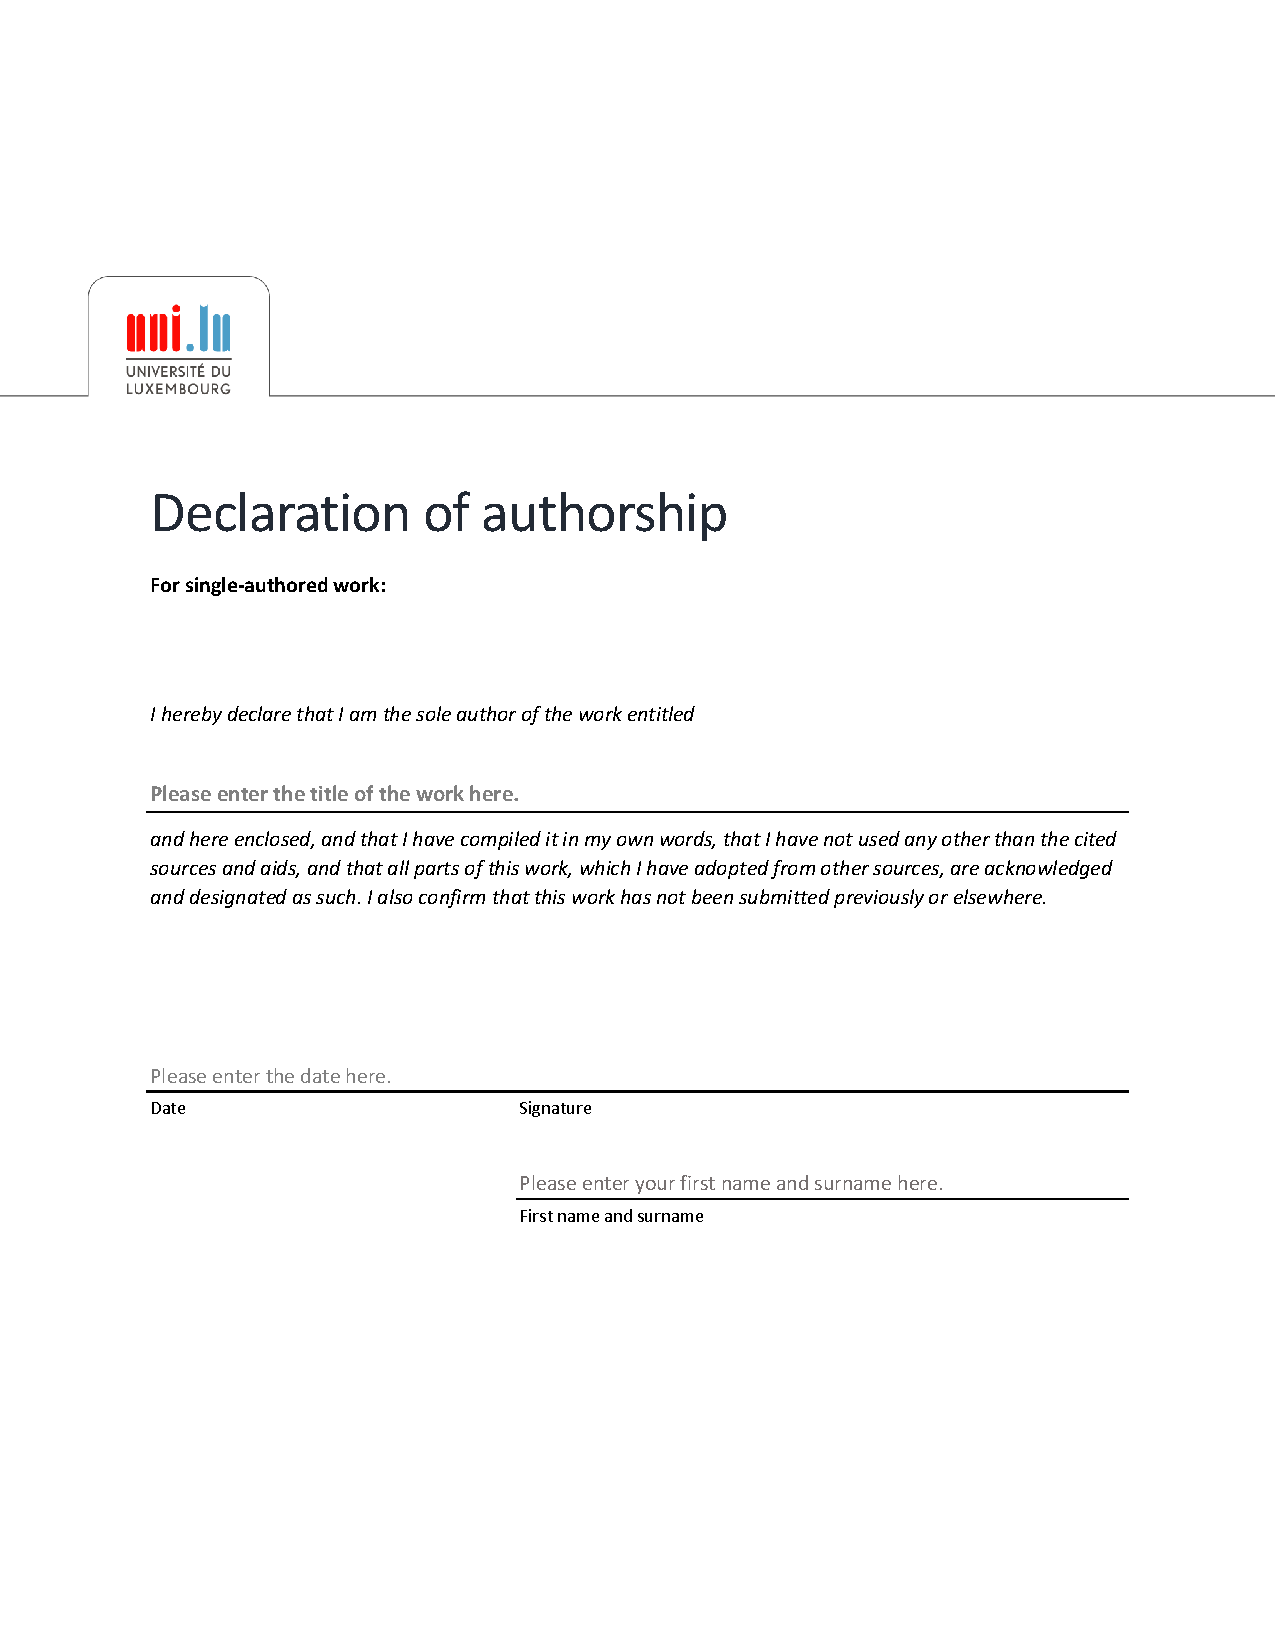
\includepdf{declaration-of-authorship.pdf}
\addcontentsline{toc}{section}{Declaration of Authorship}

\blankpage
\section*{Abstract}
\addcontentsline{toc}{section}{Abstract}

The abstract is a very brief summary of the dissertation's contents. It should be about half a page long.\footnote{Some explanations from \url{https://www.overleaf.com/latex/templates/meng-beng-msc-report-template-eee-imperial-college-london-v1-dot-3-0/qtkpngktpwpw}}

\begin{itemize}
\item Audience: technical or academic peers.
\item Language: uses discipline-specific terminology and assumes the reader has technical background knowledge.
\item Purpose: to give experts a quick overview of the work so they can decide whether to read the full document.
\end{itemize}

\textbf{Example of Abstract}\\
We propose a novel convex optimization framework for parameter identification in nonlinear dynamical systems using sparse measurements. The approach leverages structured regularization and is validated on a benchmark biochemical reaction model, showing improved accuracy and robustness compared to existing methods.\\[0.5cm]

\textbf{Structure}: You should structure your abstract as follows (around 1 line for each):
\begin{itemize}
\item What is the context of the work?
\item What is the problem?
\item Why is it an interesting problem to solve?
\item How do you solve it?
\item What are the results/contributions?
\end{itemize}
Note that usually, we tend to focus on the fourth question ``how do you solve it'', because it is where you explain your work, but an abstract shouldn't dwelve into details.

\newpage
\blankpage

\section*{Plain Language Summary}
\addcontentsline{toc}{section}{Plain Language Summary}

Also this should be about half a page long.

\begin{itemize}
\item Audience: non-experts, such as policymakers, journalists, or the general public.
\item Content: explains why the research matters, what was done, and what the implications and impact are, without technical jargon.
\item Language: clear, simple, and accessible; often includes metaphors or examples to aid understanding. Do not use acronyms.
\item Purpose: to communicate the significance and relevance of the work to a broad audience.
\end{itemize}

\textbf{Example of Plain Language Summary (for the same project in the abstract! Can you see how different this is?)}\\
Understanding how complex systems like biological reactions behave is important in medicine and engineering. We developed a new mathematical technique that can help uncover how these systems work, even if we only have limited data. This could help researchers make better predictions and design more effective treatments.


\newpage
\blankpage

\section*{Acknowledgments}
\addcontentsline{toc}{section}{Acknowledgements}

\newpage
\blankpage

\tableofcontents
\newpage
\pagenumbering{arabic}
\section{Introduction}

The introduction should be structured similarly to the abstract, but instead of one line per item, you can have one or more paragraphs.
Note that you don't need to introduce the company / laboratory in which you wrote your master thesis; this is not an internship report.
Take writing this thesis as an opportunity to think about ``What is your research question?'', what is the problem you solve.
We are usually very focussed on how to solve a task, and it is easy to lose track of what is the underlying research question.

As a requirement, you must have the following paragraph in your introduction (normally at the end):

\paragraph{Contributions}
\begin{itemize}
  \item Introduce a parallel algorithm to solve an important problem (Section~\ref{new-algo}).
  \item Experiments on a well-known benchmarks show 10\% improvement on average (Section~\ref{experiments}).
\end{itemize}

\section{Background}

Introduce the necessary background to understand your work. You are not writing a book so it is not necessary to have a 20 pages background section. However, you should attempt to be as much self-contained as possible. You can do that by only introducing theory and things that you are using later in this thesis.

\textbf{Example of reference}: \textit{Abstract interpretation} is a technique to statically analyze programs~\cite{cousot-abstract-1977}.

\section{New Parallel Algorithm}
\label{new-algo}

\section{Experimental Evaluation}
\label{experiments}

\section{Conclusion}

\newpage
\bibliographystyle{acm}
\bibliography{references.bib}

\end{document}
